\section{Experimental Apparatus}\label{apparatus.sec}

Experiment E03-103 was carried out in Hall C at the Thomas Jefferson National
Accelerator Facility (JLab)~\cite{Leemann:2001dg}. The unpolarized
electron beam from the Continuous Electron Beam Accelerator Facility was
incident on targets. The High Momentum Spectrometer (HMS) (a magnetic focusing
spectrometer) was used to detect the scattered electrons. The nominal electron
beam energy ($E$) was measured with the Hall C arc energy
measurement~\cite{XX}, the scattered momentum ($E^{'}$) and angle ($\theta$)
are reconstructed from the particle trajectory in the HMS.


 
\subsection{Experiment kinematics}\label{exptkinem.ssec}

Most of the data for the experiment were taken at 5.776 GeV beam energy with
beam currents of 30--80~$\mu A$. The cryogenic targets $^2$H, $^3$He,$^4$He
and solid targets $^9$B, $^{12}$C, $^{63}$Cu and $^{197}$Au were studied. Data
on all targets were taken at 40$\ensuremath{^\circ}$ and
50$\ensuremath{^\circ}$, and the cross section ratios with respect to
deuterium were extracted. At high $x$, the kinematics were not in the
conventional DIS region ($W^2>4\,\mathrm{GeV^2}$), so additional data were
taken for $^{12}$C and $^2$H at 8 additional kinematic settings, half at
$E$=5.776~GeV and half at 5.01~GeV, as shown in Fig.~\ref{xemkinem_fig}.

\begin{figure}[htb]
\begin{center}
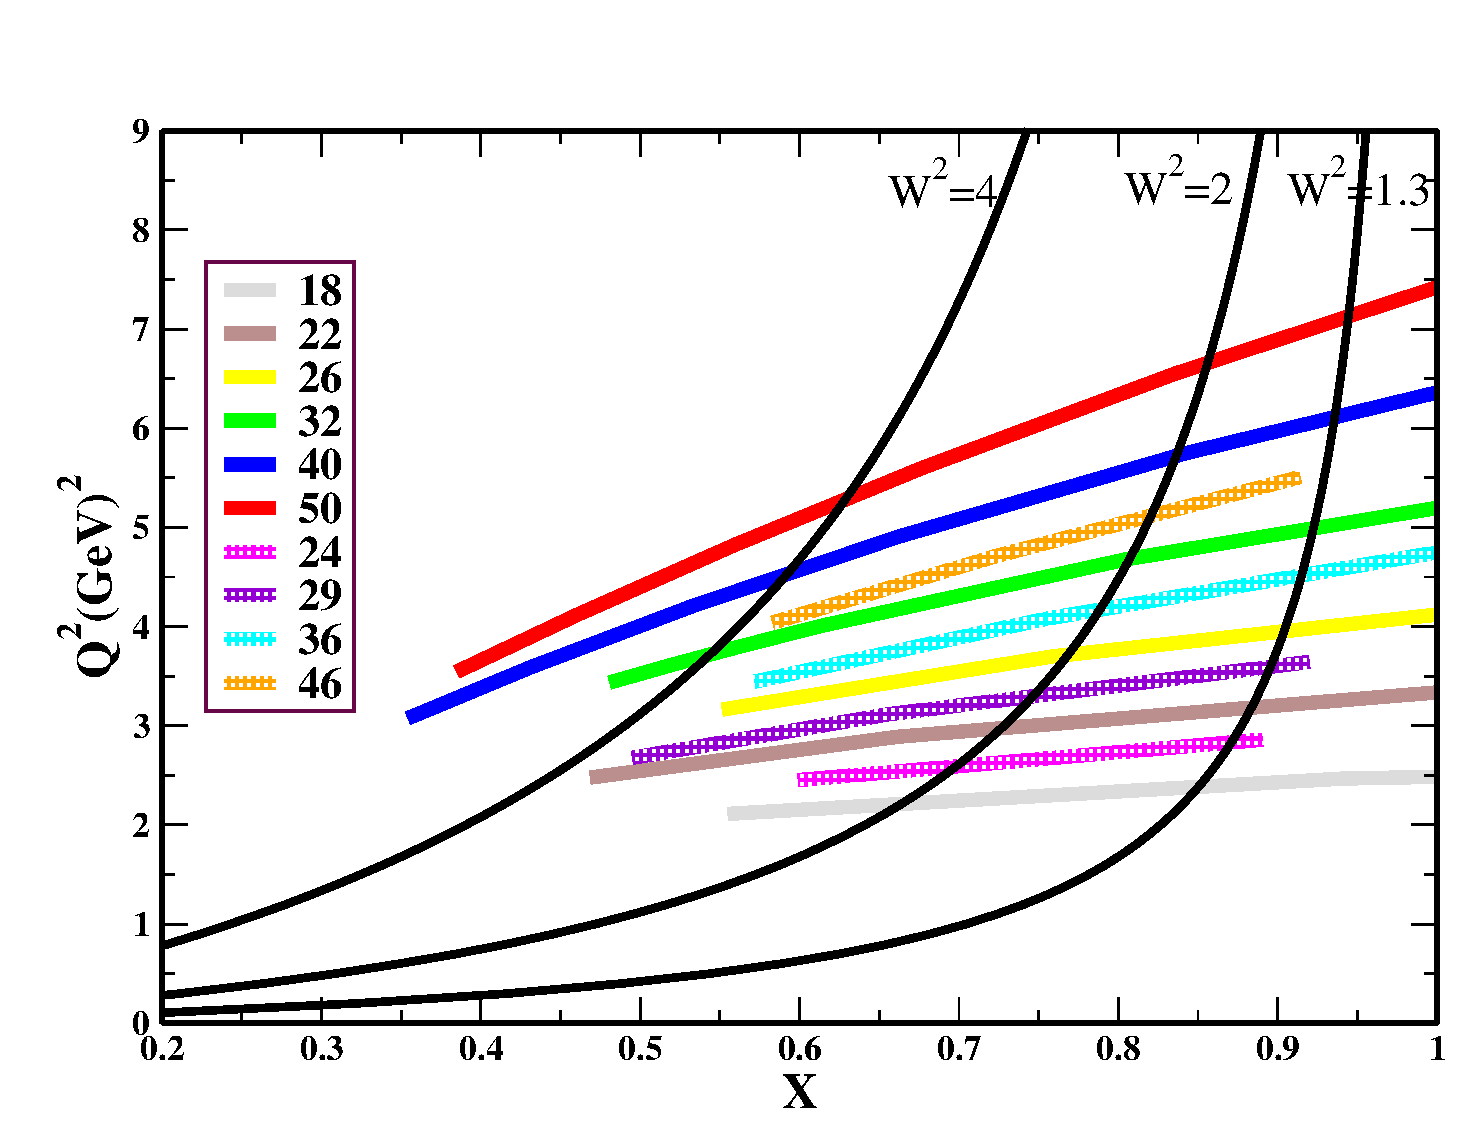
\includegraphics[height=60mm,angle=0]{plots/phasespaceXbj.eps}
\caption{(Color online) Kinematic coverage for the experiment. Contours of
constant invariant mass square are shown with black lines. Different colors
represent different angles, given in the legend. Solid lines were taken at
$E$=5.776~GeV beam energy and hatched lines at 5.01~GeV.}
\label{xemkinem_fig}
\end{center}
\end{figure}

\subsection{Targets}\label{target.ssec}

E03-103 measured inclusive electron scattering from a wide range of nuclei
using both cryogenic and solid targets. This experiment used the
standard Hall C target ladder (see Fig.~\ref{tarladder_fig}) which was placed
inside a vertical cylindrical vacuum scattering chamber. The scattering
chamber had entrance and exit openings for the beam as well as a vacuum
pumping port and several view ports. The beamline connects directly to the
scattering chamber, so the beam does not pass through any solid entrance
window. There are two cutouts on the chamber for the two spectrometers to
detect the scattered particles, which are covered with thin aluminum windows.

\begin{figure}[htb]
\begin{center}
\includegraphics[width=80mm, angle=0]{plots/target_ladder.eps}
\caption{A schematic side view of Hall C target ladder.}
\label{tarladder_fig}
\end{center}
\end{figure}

\begin{table}[htb]
\begin{center}
\caption{Nominal cryotarget dimensions. Here, $\left<t\right>$ represents the
average offset-corrected cryogen in the path of the beam and R.R.L is the
relative radiation length which represents the amount of material in the path
of the
beam.\label{cryotarthick_tab}}
\begin{tabular}{|l|c|c|c|c|c|}
\hline
Target & $\left<t\right>$ & Density & Areal thickness &R.R.L & Purity\\ 
& (cm) & (g/cm$^3$) & (g/cm$^2$) &($\%$) &($\%$)\\
\hline
$^1$H  & 3.865 & 0.0723 & 0.2794(36) & 0.456 &99.99\\
$^2$H  & 3.860 & 0.167  & 0.6446(83) & 0.526 &99.95\\
$^3$He & 3.865 & 0.0708 & 0.2736(51) & 0.419 &99.9\\
$^4$He & 3.873 & 0.135  & 0.5229(85) & 0.554 &99.99\\
\hline
\end{tabular}
\end{center}
\end{table}

The target assembly contains several loops for cryogenic targets and the solid
target ladder was attached above the optics sled. The target stack can be
raised or lowered by an actuator in order to put the desired target in the
beam path. The cryogenic targets were contained in vertical cylindrical Al cans
with a diameter of $\approx 4$ cm. Each loop consisted of a circulation fan, a
target cell, heat exchangers and high powered heaters. The target liquid in
each loop was cooled with helium gas using a heat exchanger. The liquid moved
continuously through the heat exchanger, to the target cell and back. A high
power heater regulated the temperature of the cryogenic targets, compensating
for the power deposition by the beam during low current or beam off periods.
Solid targets were attached above the optics sled and all the foils in the
solid target ladder were separated vertically.

The optics sled contained a dummy target, which consisted of two aluminum
foils (aluminum alloy Al-6061-T6) placed $\sim4$ cm apart. These dummy targets
mimicked the cell walls of the cryogenic target and facilitated the
measurement of the background originating from the cell walls. The dummy
targets were flat aluminum foils and were approximately 8 times thicker than
the walls of liquid targets to reduce the time needed for background
measurement.


\begin{table}[htb]
\begin{center}
\caption{Solid target dimensions, radiation length, and purity. Here, Al(1)
and Al(2) represents the aluminum foils which mimicked the cell walls of
cryogenic target.}
\label{solidltarthick_tab}
\begin{tabular}{|l|c|c|c|c|}
\hline
Target & Density &Areal thickness & R. R. L. & Purity\\ 
& (g/cm$^3$) & (g/cm$^2$) &($\%$) & ($\%$)\\
\hline
Be    & 1.848 & 1.8703(94) & 2.87 & 99.0 \\
C     & 2.265 & 0.6667(40) & 1.56 & 99.95\\
Cu    & 8.96  & 0.7986(40) & 6.21 & 99.995 \\
Au    & 19.32 & 0.3795(38) & 5.88 & 99.999\\
Al(1) & 2.699 & 0.2626(13) & 1.09 & 98.0\\
Al(2) & 2.699 & 0.2633(13) & 1.10 & 98.0\\
\hline
\end{tabular}
\end{center}
\end{table}

Areal thicknesses of the cryotargets were computed (see
Table~\ref{cryotarthick_tab}) from the target density and the length of the
cryogen in the path of the beam. Since the target cans are cylindrical, the
effective target length seen by the beam differs from the diameter of the can
if the beam does not intersect the geometrical center of the targets, and a
correction accounting for beam offset is applied run-by-run. The target
density was calculated using the knowledge of temperature and pressure.
Fluctuations in the beam position can also affect the effective target length
over the course of the run. This was computed on a run by run basis and
applied to all the cryotargets.

Thicknesses of the solid targets were calculated using measurements of the
mass and area of the targets. For solid targets, there is an uncertainty in
the effective thickness due to uncertainty in angle of the target relative to
beam direction, but this is estimated to be $<0.01\%$. Solid targets used in
the experiment and their dimensions are given in
Table~\ref{solidltarthick_tab}.  No correction is applied for the $\sim$1\%
contamination of the $^9$Be target, as the cross section per nucleon for $^9$Be
and heavier nuclei differs at the few percent level, so the correction is
typically $\ll$0.1\%.


\subsection{High-Momentum Spectrometer}\label{hms.ssec}

E03-103 used the HMS to detect the scattered electrons from the interaction
vertex. The HMS is a $25\degree$ vertical-bend spectrometer that consists of
three quadrupole magnets, one dipole magnet and a detector package. The
detectors are housed inside a concrete enclosure and this shield hut is
mounted on a steel carriage which can be rotated on a pair of concentric rails
to the desired scattering angle.  An octagonal collimator is placed before the
entrance to the first magnet which is used to define the acceptance for a
short target for particles within approximately 10\% of the central momentum
setting. A schematic side view of the HMS is shown in
Figure~\ref{hmsside_fig}. All magnets in the HMS are superconducting and are
cooled with 4K liquid helium. The focusing properties and acceptance of the
HMS are determined by the quadrupole magnets, and the central momentum is
determined by the dipole. See Ref.~\cite{johna_thesis, Dutta:2003yt} for more
details on the spectrometer and detector package.

There are two vertical drift chambers in the HMS located at the front of the
detector stack~\cite{baker95}. The drift chambers are used to find the
position and trajectory of the particle at the focal plane, which are used to
reconstruct the position and momentum of the scattered particle at the
interaction vertex. Two sets of $x-y$ scintillators hodoscopes were used for
triggering and time-of-flight measurements~\cite{??}. The detector stack also
contains a threshold gas $\mathrm{\check{C}erenkov}$ counter used for electron
identification~\cite{??}. The HMS $\mathrm{\check{C}erenkov}$ detector is a large
cylindrical tank (inner diameter $\approx 150$ cm and length $\approx 165$
cm). It has two front reflecting mirrors which focus the light onto two PMTs.
The circular ends of the tank are covered with 0.1 cm aluminum windows. For
E03-103, the detector was filled with 5.15 psi ($\sim 0.35$ atmospheres) of
Perfluorobutane ($\mathrm{C_4F_{10}}$) at room temperature. At this pressure
and temperature, the index of refraction of the gas is 1.00050, yielding
a threshold momentum of 16 MeV for electrons and 4.4 GeV for pions. The pion
threshold was above the momentum range of E03-103 except for the lowest
angles, where the $\pi$/e ratio is lower and the separation between electrons
and pions in the calorimeter is sufficient to yield a negligible pion
background.

A lead glass calorimeter detector~\cite{mkrtchyan13} was used in conjunction
with the $\mathrm{\check{C}erenkov}$ detector for electron identification. The
HMS calorimeter consists of 10 cm$\times$10 cm$\times$70 cm blocks of TF-1 lead
glass, positioned at the rear of the detector hut. The blocks are arranged in
four layers with 13 blocks per layer for a total thickness of 16 radiation
lengths, along the particle direction.  Electrons or positrons entering the
calorimeter deposit their entire energy, and the normalized energy spectrum,
$E_{cal}/E^{'}$, is peaked around 1. Pions typically deposit $\sim 300 $ MeV
in the calorimeter and the $E_{cal}/E^{'}$ distribution peaks around 0.3
GeV/$E^{'}$.

\begin{figure}[htb]
\begin{center}
\includegraphics[height=75mm, angle=270]{plots/hmssideview.ps}
\caption [Side view of the HMS] {A schematic side view of the HMS.}
\label{hmsside_fig}
\end{center}
\end{figure}

